\documentclass[11pt]{article}
\usepackage{amsmath}
%\usepackage{extsizes}
\usepackage{amsmath,amssymb}
%\usepackage{omegavn,ocmrvn}
%\usepackage[utf8x]{inputenc}
\usepackage[utf8]{vietnam}

\usepackage{framed}
\usepackage[most]{tcolorbox}
\usepackage{xcolor}
\colorlet{shadecolor}{orange!15}


\usepackage{longtable}
\usepackage{answers}
\usepackage{graphicx}
\usepackage{array}
\usepackage{pifont}
\usepackage{picinpar}
\usepackage{enumerate}
\usepackage[top=3.0cm, bottom=3.5cm, left=3.5cm, right=2.5cm] {geometry}
\usepackage{hyperref}


\newtheorem{bt}{Câu}
\newcommand{\RR}{\mathbb R}
\Newassociation{sol}{Solution}{ans}
\newtheorem{ex}{Câu}
\renewcommand{\solutionstyle}[1]{\textbf{ #1}.}


\begin{document}
% \noindent
\begin{tabular*}
{\linewidth}{c>{\centering\hspace{0pt}} p{.7\textwidth}}
Trường ĐHKHTN, ĐHQGHN & {\bf Học Kỳ 1 (2018-2019)}
\tabularnewline
K61 TTƯD & {\bf Kiểm tra cuối kỳ - Đề 1 - Bài mẫu}

\tabularnewline
\rule{1in}{1pt}  \small  & \rule{2in}{1pt} %(Due date:)
\tabularnewline

%  \tabularnewline
%  &(Đề thi có 1 trang)
\end{tabular*}
%
% \Opensolutionfile{ans}[ans1]

\begin{shaded}
Đây chỉ là một mẫu đề thi thầy soạn dựa trên giới hạn của thầy Hiếu, không phải đề thi thật và không có phần nào trùng với đề thi thật.
\end{shaded}

\begin{bt} % Exercise 8, Atkinson/Han p.107
a) Các phép lặp sau có hội tụ đến $\alpha$ hay không? Nếu hội tụ, hãy xác định tốc độ hội tụ, cho $x_0$ đủ gần $\alpha$.
%
\[  a) \  x_{n+1} = \cfrac{15 x_n^2-24x_n+13}{4x_n} \ , \ \alpha=1, \hskip 4cm b) \  x_{n+1} = \cfrac{3}{4} x_n + \cfrac{1}{x_n^3} \ , \ \alpha=\sqrt{2}.\]
%
b) Tìm số bước lặp cần thiết để nhận được xấp xỉ với sai số tuyệt đối không quá $1e-5$, với $x_0 = \alpha + 1e-1$. \\
c) Viết công thức đánh giá sai số hậu nghiệm và áp dụng để đánh giá sai số của $x_3$, với $x_0$ như câu $b$.
\end{bt}

\begin{bt}(3đ) % Che/Kincaid 07, page 503, Ex. 16
Độ nhớt của một chất lưu là thông số đại diện cho ma sát trong của dòng chảy. Độ nhớt được biểu diễn qua một hàm bậc hai của nhiệt độ T, tức là $V = a + bT + cT^2$. Hãy dùng cả 2 phương pháp "lập phương trình chính tắc" và "trực giao hóa ma trận" để tìm các hệ số của hàm xấp xỉ tốt nhất bảng số liệu sau theo phương pháp bình phương tối thiểu.
%
\begin{center}
	\begin{tabular}[7]{l|l|l|l|l|l|l|l}
		T & 1    & 2    & 3    & 4    & 5    & 6    & 7 \\ \hline
		V & 2.31 & 2.01 & 1.80 & 1.66 & 1.55 & 1.47 & 1.41.
	\end{tabular}	
\end{center}
% 
\end{bt}

\begin{bt}
Cho hệ phương trình sau
%
\begin{align*}
2 x_1 + 4 x_2 + 3x_3   &= 3, \\
3 x_1 + x_2 - 2 x_3    &= 3, \\
4 x_1 + 11 x_2 + 7 x_3 &= 4. 
\end{align*}
%
a) Hãy đi tìm phân tích LU có pivot như trong phân tích phần tử trội.\\
b) Giải hệ phương trình trên bằng phương pháp phần tử trội.
\end{bt}

\newpage

\begin{bt}
	Cho bài toán Cauchy
\end{bt}

\begin{figure}[h!]
	\centering
	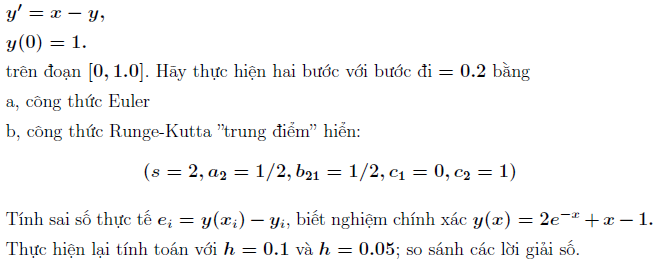
\includegraphics[scale = 0.9]{7}
\end{figure}

\begin{shaded}
Trong Đề 1 bài tập 3 có thể được thay bằng giải hệ bằng phân tích Cholesky như sau.
\end{shaded}

\begin{bt}
	Cho hệ phương trình dạng $Ax=b$ với ma trận hệ số vế trái là đối xứng, xác định dương như sau. 
	%
	\begin{align*}
	4 x_1 - 2 x_2 + 4 x_3   &= b_1, \\
	-2 x_1 + 5 x_2 - 4 x_3  &= b_2, \\
	4 x_1  -4 x_2 + 6 x_3   &= b_3. 
	\end{align*}
	%
	a) Hãy tìm phân tích Cholesky của ma trận A. \\
	b) Sử dụng phương pháp Cholesky để tìm nghiệm của hệ phương trình trên.
\end{bt}

\centerline{———————————Hết——————————-}

\end{document}

\vspace{1cm}
\noindent{\bf Chú ý:} {\it Cán bộ coi thi không giải thích gì thêm}\\
\Closesolutionfile{ans}
\newpage
\begin{center}
{\LARGE{\bf ĐÁP ÁN}}
\end{center}

\begin{sol}
	\begin{figure}[h!]
		\centering
		\includegraphics[width=0.8\linewidth]{Solution1/Sol4_1.png}
		%\caption{}
		\label{fig:Sol4}
	\end{figure}
	Exercise 7: Convergence order is 3.	
\end{sol}

   
\end{document}



